\documentclass[aspectratio=169]{beamer}
\useoutertheme[progressbar=frametitle]{metropolis}
\useinnertheme{metropolis}
\definecolor{nabgray}{rgb}{0.6,0.59,0.61}
\usecolortheme[named=nabgray]{structure}

\usepackage{tikz}
\usepackage[utf8]{inputenc}
\usepackage[spanish]{babel}
\usepackage{fontspec}
\usepackage{ulem}

\setmonofont{JetBrains Mono}
\setmainfont{Roboto}
\setsansfont{Roboto}


\usepackage{smartdiagram}
\usepackage{qtree}
\usepackage{verbatim}
\usepackage{svg}
\usepackage{graphicx}
\usepackage{color}


\definecolor{lightgray}{rgb}{0.95, 0.95, 0.95}
\definecolor{darkgray}{rgb}{0.4, 0.4, 0.4}
%\definecolor{purple}{rgb}{0.65, 0.12, 0.82}
\definecolor{editorGray}{rgb}{0.95, 0.95, 0.95}
\definecolor{editorOcher}{rgb}{1, 0.5, 0} % #FF7F00 -> rgb(239, 169, 0)
\definecolor{editorGreen}{rgb}{0, 0.5, 0} % #007C00 -> rgb(0, 124, 0)
\definecolor{orange}{rgb}{1,0.45,0.13}
\definecolor{olive}{rgb}{0.17,0.59,0.20}
\definecolor{brown}{rgb}{0.69,0.31,0.31}
\definecolor{purple}{rgb}{0.38,0.18,0.81}
\definecolor{lightblue}{rgb}{0.1,0.57,0.7}
\definecolor{lightred}{rgb}{1,0.4,0.5}
\definecolor{ocherCode}{rgb}{1, 0.5, 0} % #FF7F00 -> rgb(239, 169, 0)
\definecolor{blueCode}{rgb}{0, 0, 0.93} % #0000EE -> rgb(0, 0, 238)
\definecolor{greenCode}{rgb}{0, 0.6, 0} % #009900 -> rgb(0, 153, 0)


\usepackage{upquote}
\usepackage{listings}
\lstdefinelanguage{JavaScript}{
    morekeywords=[1]{break, continue, delete, else, for, function, if, in,
        new, return, this, typeof, var, void, while, with},
    % Literals, primitive types, and reference types.
    morekeywords=[2]{false, null, true, boolean, number, undefined,
        Array, Boolean, Date, Math, Number, String, Object},
    % Built-ins.
    morekeywords=[3]{eval, parseInt, parseFloat, escape, unescape},
    % Basic design
    backgroundcolor=\color{lightgray},
    basicstyle={\small\ttfamily},
    frame=l,
    keywordstyle=\footnotesize\color{blue},
    escapeinside={<@}{@>},
    breaklines=true,
    % Line numbers
    xleftmargin={0.75cm},
    numbers=left,
    stepnumber=1,
    firstnumber=1,
    numberfirstline=true
    % Code design
    identifierstyle=\color{black},
    keywordstyle=\color{ocherCode}\bfseries,
    ndkeywordstyle=\color{greenCode}\bfseries,
    stringstyle=\color{ocherCode}\ttfamily,
    commentstyle=\color{darkgray}\ttfamily,
    tabsize=2,
    showtabs=true,
    showspaces=false,
    showstringspaces=false,
    extendedchars=true,
    breaklines=true
}[keywords, comments, strings]

\colorlet{punct}{red!60!black}
\definecolor{background}{HTML}{EEEEEE}
\definecolor{delim}{RGB}{20,105,176}
\colorlet{numb}{magenta!60!black}

\lstdefinelanguage{json}{
    basicstyle=\normalfont\ttfamily,
    numbers=left,
    numberstyle=\scriptsize,
    stepnumber=1,
    numbersep=8pt,
    showstringspaces=false,
    breaklines=true,
    frame=lines,
    literate=
    *{0}{{{\color{numb}0}}}{1}
    {1}{{{\color{numb}1}}}{1}
    {2}{{{\color{numb}2}}}{1}
    {3}{{{\color{numb}3}}}{1}
    {4}{{{\color{numb}4}}}{1}
    {5}{{{\color{numb}5}}}{1}
    {6}{{{\color{numb}6}}}{1}
    {7}{{{\color{numb}7}}}{1}
    {8}{{{\color{numb}8}}}{1}
    {9}{{{\color{numb}9}}}{1}
    {:}{{{\color{punct}{:}}}}{1}
    {,}{{{\color{punct}{,}}}}{1}
    {\{}{{{\color{delim}{\{}}}}{1}
    {\}}{{{\color{delim}{\}}}}}{1}
    {[}{{{\color{delim}{[}}}}{1}
    {]}{{{\color{delim}{]}}}}{1},
}
\lstset{language=java,
    basicstyle=\footnotesize\ttfamily,
    keywordstyle=\footnotesize\color{blue}\ttfamily,
}


\usebackgroundtemplate%
{%
    
\includegraphics[width=\paperwidth]{Images/Contenido}%
}


\title{Consejos y el camino del desarrollador de software}
\author{Víctor Orozco}
\institute{Academik}
\date{\today}
\begin{document}


{
	\usebackgroundtemplate{
\includegraphics[width=\paperwidth]{Images/portada}}
	\setbeamercolor{frametitle}{fg=red}
	\usebeamercolor[fg]{normal text}
	\frame{\titlepage}
}


{
	\usebackgroundtemplate{
\includegraphics[width=\paperwidth]{Images/separador}}
	\setbeamercolor{normal text}{fg=white}
	\setbeamercolor{frametitle}{fg=red}
	\usebeamercolor[fg]{normal text}
	\section{¿Que hace un desarrollador de software?}
}

\begin{frame}
    \huge ¡Programar!
\end{frame}

\begin{frame}{Programar}


    \begin{columns}[T] % contents are top vertically aligned
	     \begin{column}[T]{0.5\textwidth} % each column can also be its own environment
			    \begin{itemize}[<+->]
                       \item Entender problemas con visión de sistemas (integral)
                       \item Planificar la mejor forma de resolver un problema
                       \item Decirle a un sistema informático como realizar su tarea a través de lenguajes de programación
                       \item Probar el funcionamiento de un sistema informático
                       \item Ser el responsable que todo lo anterior funcione (3-10 años)
                \end{itemize}
	     \end{column}
	     \begin{column}[T]{4cm} % alternative top-align that's better for graphics
   			\begin{figure}
                       \centering
                       
\includegraphics[width=\linewidth]{Images/yo}
                   \end{figure}

	     \end{column}
     \end{columns}
\end{frame}

{
	\usebackgroundtemplate{
\includegraphics[width=\paperwidth]{Images/separador}}
	\setbeamercolor{normal text}{fg=white}
	\setbeamercolor{frametitle}{fg=red}
	\usebeamercolor[fg]{normal text}
	\section{¿Porqué aprender a desarollar software?}
}





\begin{frame}{Oportunidades}

            \begin{figure}
                \centering
                
\includegraphics[width=\linewidth]{Images/cangrejo}
            \end{figure}
\end{frame}

\begin{frame}{Oportunidades}

            \begin{figure}
                \centering
                
\includegraphics[width=\linewidth]{Images/trabajo}
            \end{figure}
\end{frame}

\begin{frame}{Oportunidades}

            \begin{figure}
                \centering
                
\includegraphics[width=0.7\linewidth]{Images/jobs}
            \end{figure}
\end{frame}


{
	\usebackgroundtemplate{
\includegraphics[width=\paperwidth]{Images/separador}}
	\setbeamercolor{normal text}{fg=white}
	\setbeamercolor{frametitle}{fg=red}
	\usebeamercolor[fg]{normal text}
	\section{¿Quien puede ser un desarrollador de software?}
}





\begin{frame}{Desarrollador}
    \begin{alertblock}{Hecho importante}
    Ni todo desarrollador de software es ingeniero, ni todo ingeniero sabe programar. De hecho la mayoría de ingenieros solo lo hace a un nivel básico hasta que sale del área.
    \end{alertblock}
    Lo que si es un hecho es que es una profesión que requiere educación y practica constante
\end{frame}

\begin{frame}[fragile,c]{Desarrollador}

\begin{columns}[T] % contents are top vertically aligned
	     \begin{column}[T]{7cm} % each column can also be its own environment
				\smartdiagramset{
                    bubble node size =2.5cm,
                    bubble center node font = \small,
                    bubble node font = \tiny,
                    distance center/other bubbles = 0.7cm,
                    }
                    \smartdiagram[bubble diagram]{Habilidades,
                      Curiosidad, Paciencia, Lectura, Lógica, Resolución de problemas}

	     \end{column}
	     \begin{column}[T]{4cm} % alternative top-align that's better for graphics
             Opciones de formación
			\begin{itemize}
    			\item Cursos cortos
                \item Boot-camps
                \item Universidad

			\end{itemize}

	     \end{column}
     \end{columns}

\end{frame}


\begin{frame}[fragile,c]{Desarrollador - No todos son iguales}

 \begin{figure}
        \centering
        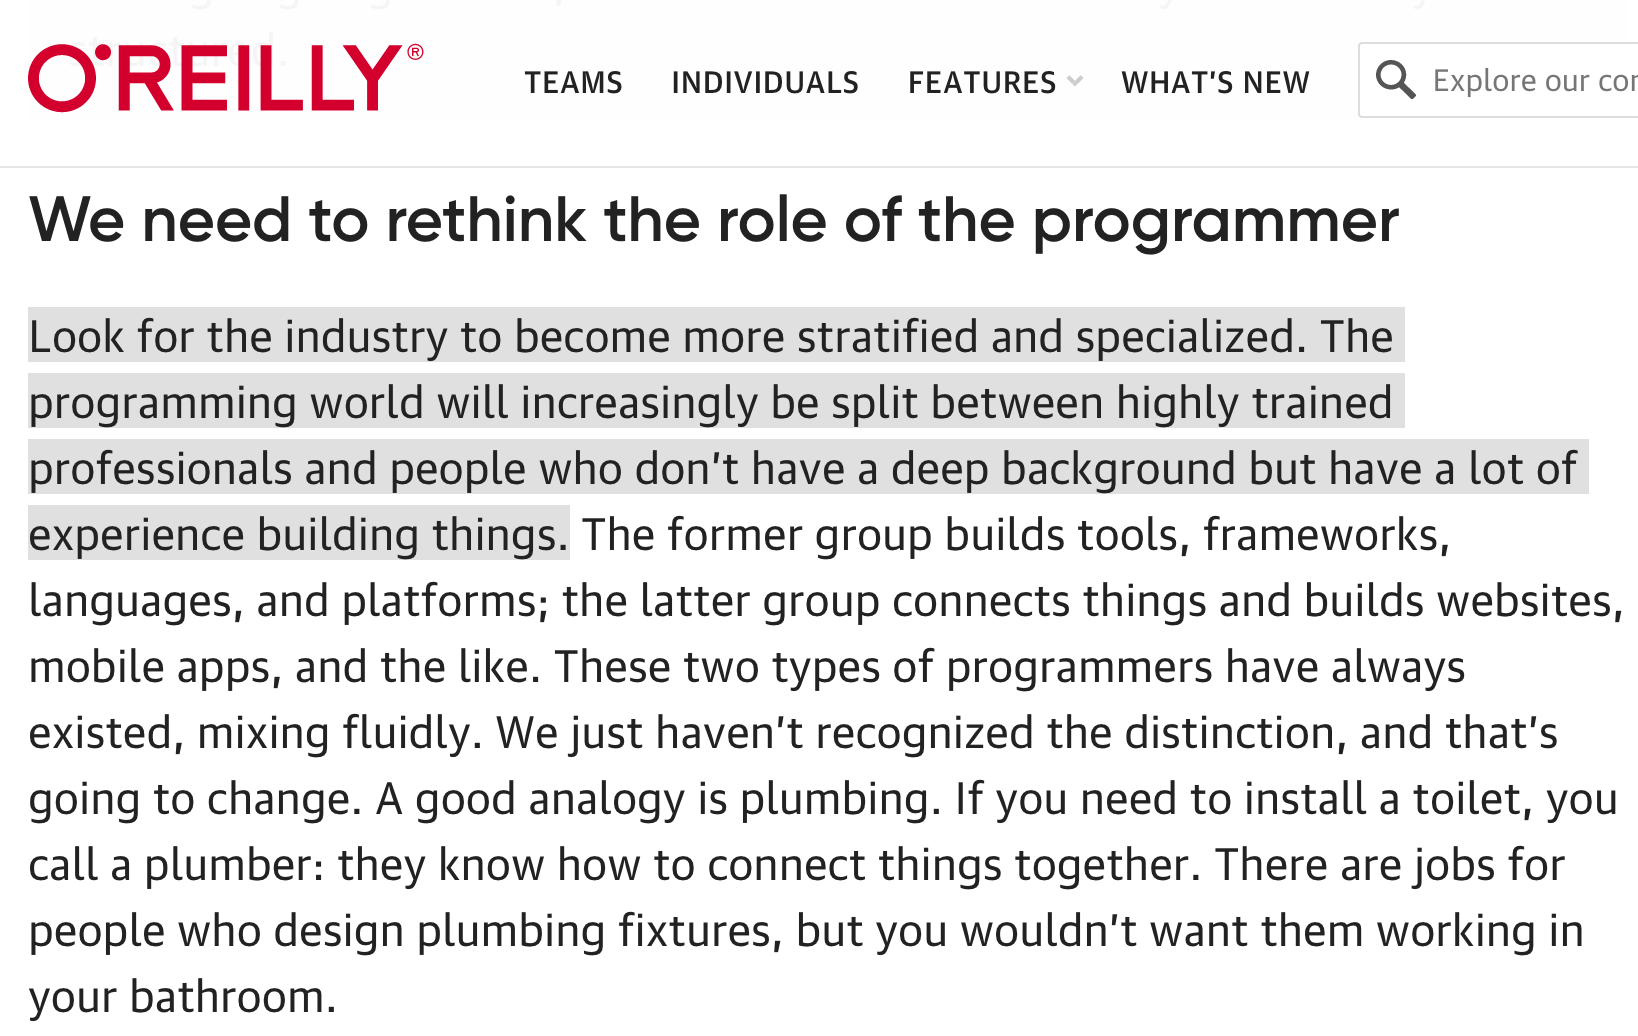
\includegraphics[width=0.9\linewidth]{Images/oreilly}
    \end{figure}
\end{frame}


{
	\usebackgroundtemplate{
\includegraphics[width=\paperwidth]{Images/separador}}
	\setbeamercolor{normal text}{fg=white}
	\setbeamercolor{frametitle}{fg=red}
	\usebeamercolor[fg]{normal text}
	\section{Tipos de programadores}
}




\begin{frame}{Backend vs frontend}
	\begin{figure}
		\centering
		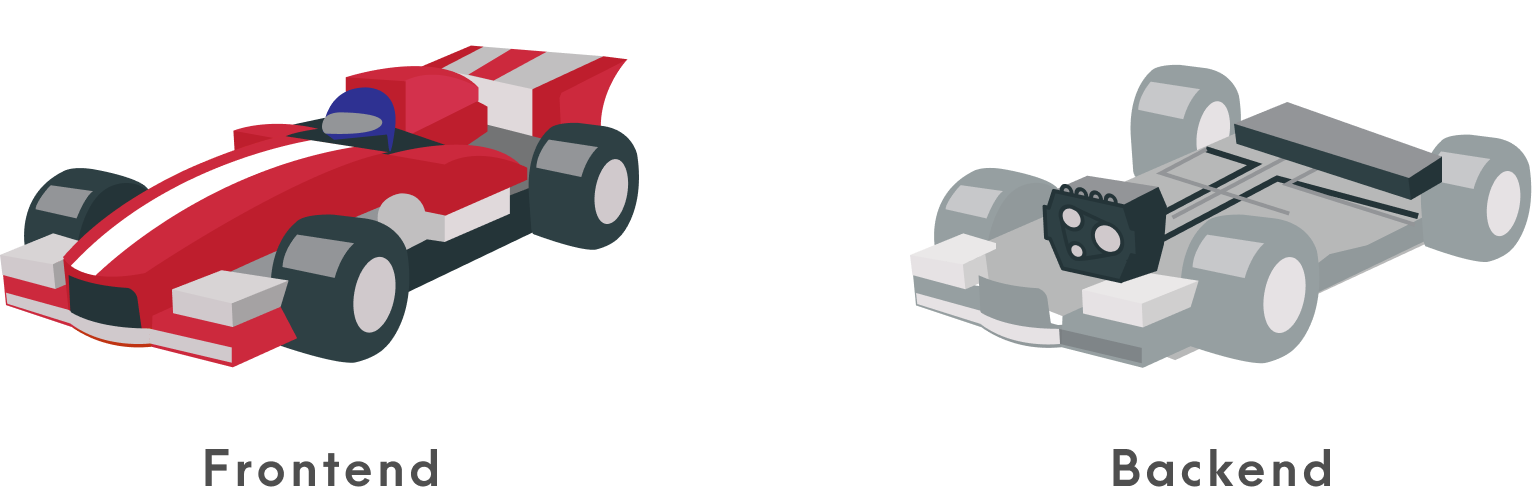
\includegraphics[width=\linewidth]{Images/backvsfront}
	\end{figure}
\end{frame}



\begin{frame}{Backend vs mobile}
	\begin{figure}
		\centering
		
\includegraphics[width=\linewidth]{Images/backvsmobile.png}
	\end{figure}
\end{frame}


{
	\usebackgroundtemplate{
\includegraphics[width=\paperwidth]{Images/separador}}
	\setbeamercolor{normal text}{fg=white}
	\setbeamercolor{frametitle}{fg=red}
	\usebeamercolor[fg]{normal text}
	\section{¿Como deberia aprender?}
}





\begin{frame}{Elementos de aprendizaje}
    \smartdiagramset{
                        bubble node size =2.5cm,
                        bubble center node font = \small,
                        bubble node font = \tiny,
                        distance center/other bubbles = 0.7cm,
                        }
                        \smartdiagram[bubble diagram]{Programar,
                          Lenguaje, Lógica, Herramientas, Frameworks}
\end{frame}

\begin{frame}{¿Como aprender Java?}
     \begin{figure}
            \centering
            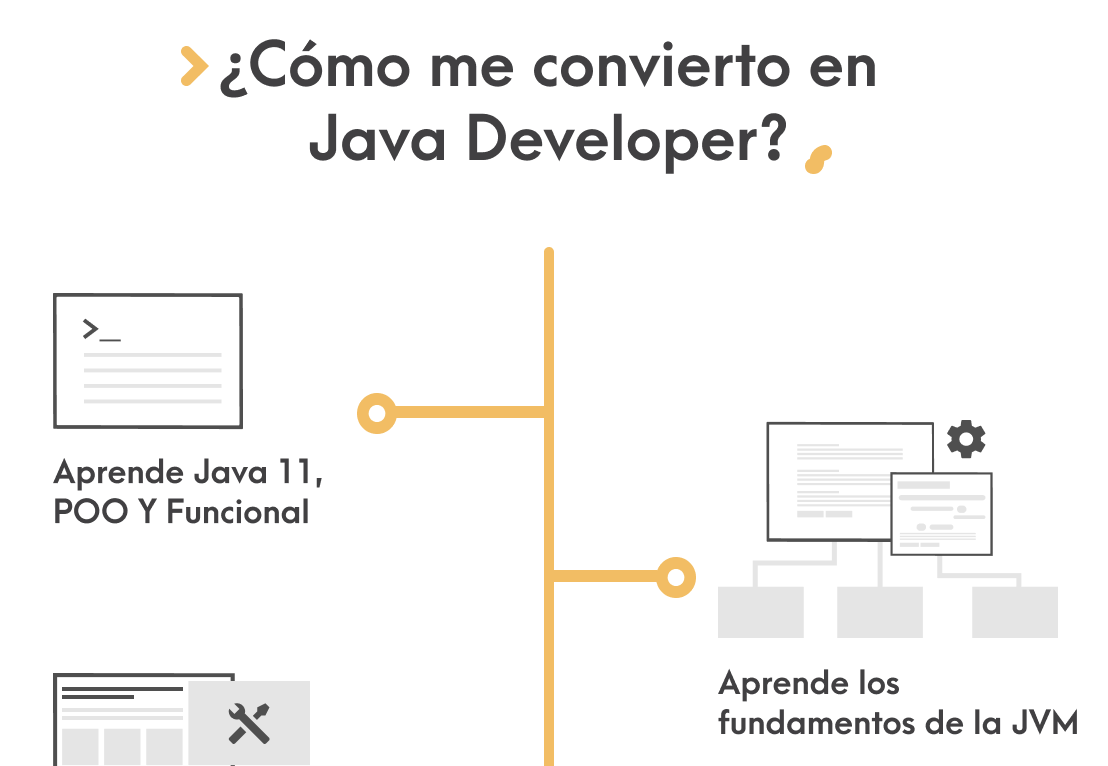
\includegraphics[width=0.7\linewidth]{Images/camino1}
        \end{figure}
\end{frame}


\begin{frame}{¿Como aprender Java?}
     \begin{figure}
            \centering
            
\includegraphics[width=0.7\linewidth]{Images/camino2}
        \end{figure}
\end{frame}

\begin{frame}{¿Como aprender Java?}
     \begin{figure}
            \centering
            
\includegraphics[width=0.7\linewidth]{Images/camino3}
        \end{figure}
\end{frame}

{
	\usebackgroundtemplate{
\includegraphics[width=\paperwidth]{Images/separador}}
	\setbeamercolor{normal text}{fg=white}
	\setbeamercolor{frametitle}{fg=red}
	\usebeamercolor[fg]{normal text}
	\section{¿Hay niveles?}
}


\begin{frame}[fragile,c]{Niveles}

 \begin{figure}
        \centering
        
\includegraphics[width=0.7\linewidth]{Images/niveles1}
    \end{figure}
\end{frame}

\begin{frame}[fragile,c]{Niveles}

 \begin{figure}
        \centering
        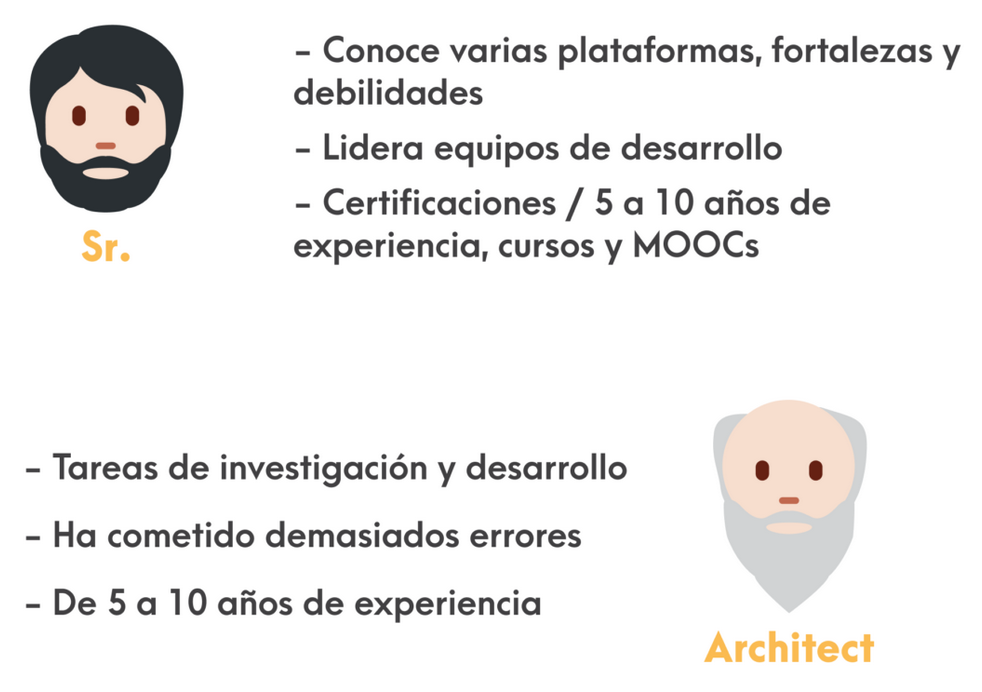
\includegraphics[width=0.7\linewidth]{Images/niveles2}
    \end{figure}
\end{frame}

\begin{frame}{Principios de sobrevivencia - Redmonk}
	\begin{figure}
		\centering
		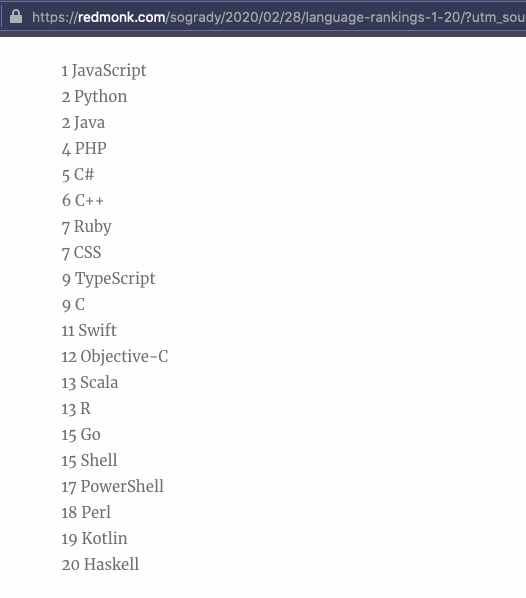
\includegraphics[width=0.9\linewidth]{Images/redmonk}
	\end{figure}
\end{frame}

\begin{frame}{Principios de sobrevivencia - Tiobe}
	\begin{figure}
		\centering
		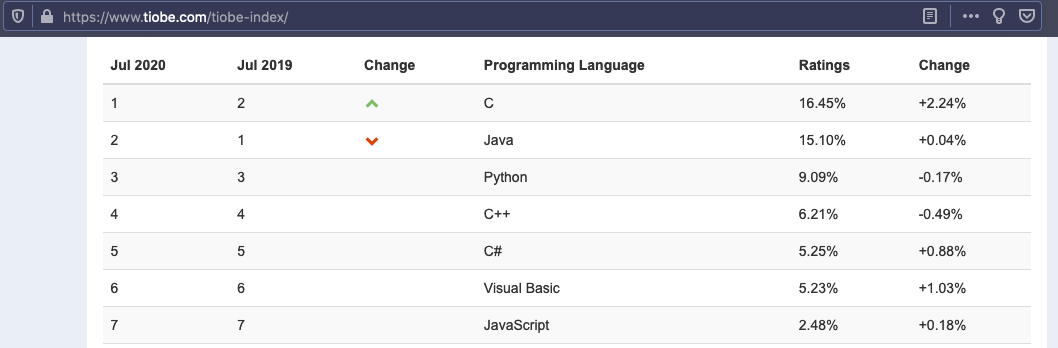
\includegraphics[width=0.9\linewidth]{Images/tiobe}
	\end{figure}
\end{frame}

\begin{frame}{Principios de sobrevivencia - IEEE}
    \begin{figure}
        \centering
        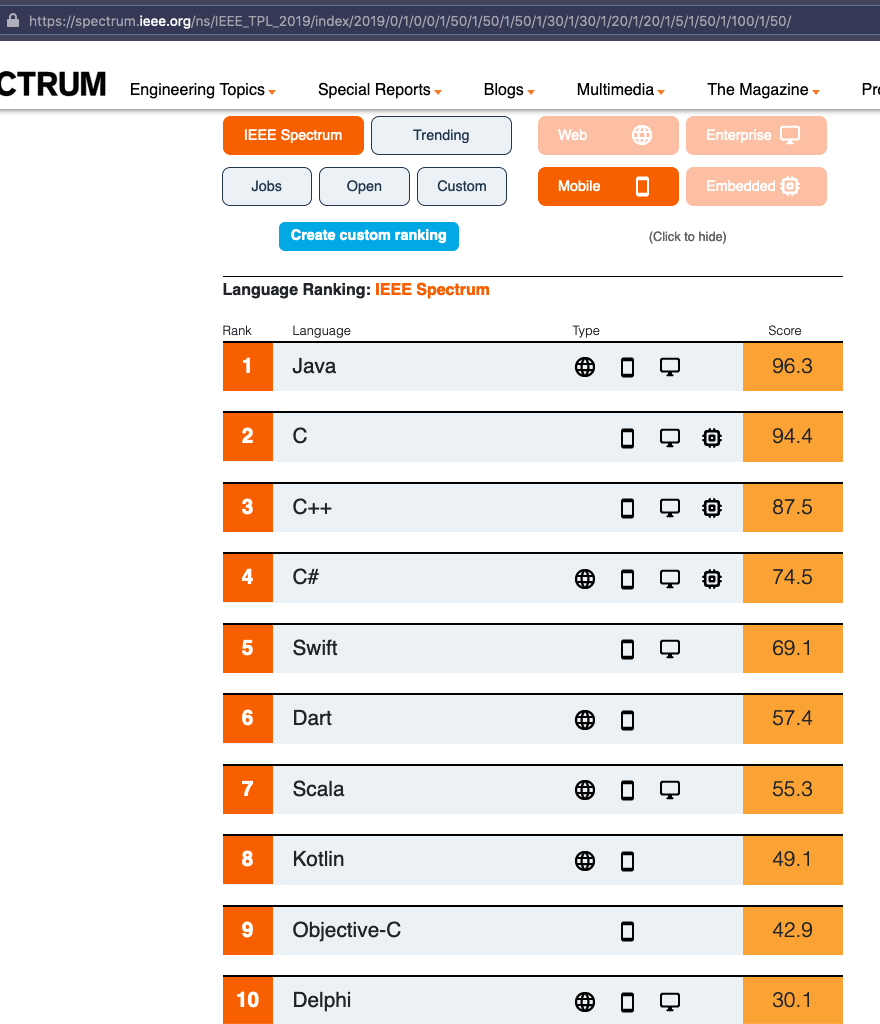
\includegraphics[width=0.5\linewidth]{Images/ieeemobile}
    \end{figure}
\end{frame}

\begin{frame}{Principios de sobrevivencia - IEEE}
    \begin{figure}
        \centering
        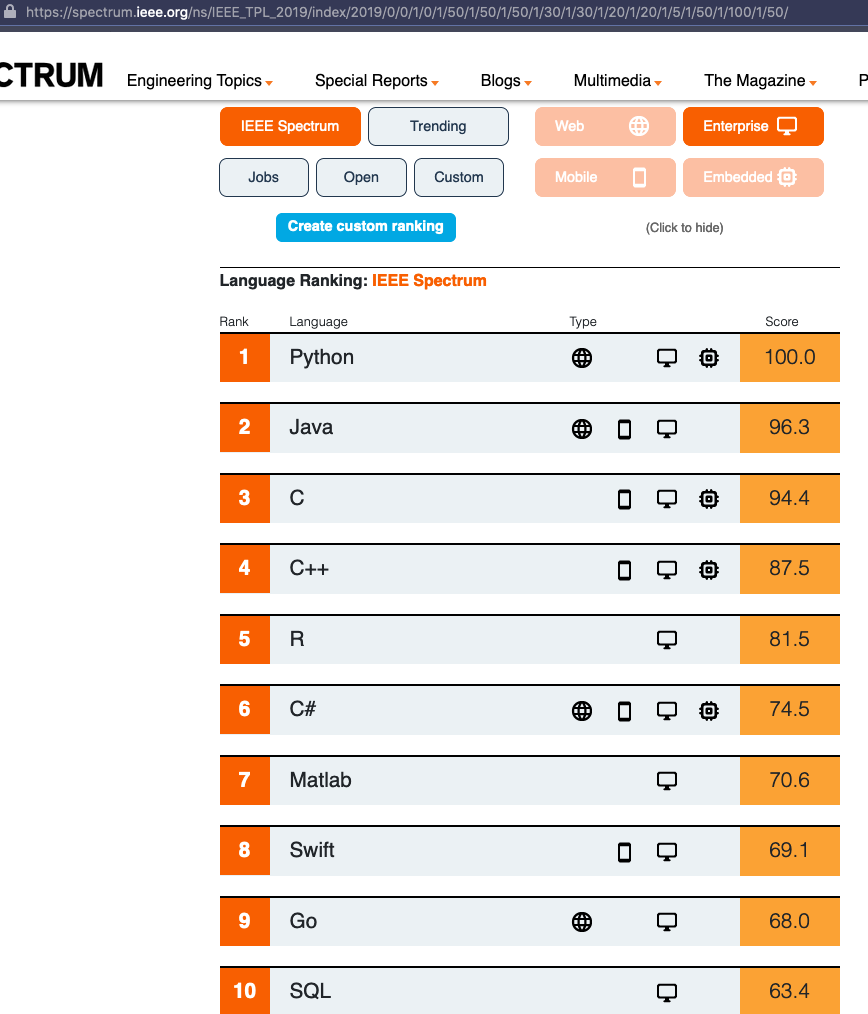
\includegraphics[width=0.5\linewidth]{Images/ieeeenterpise}
    \end{figure}
\end{frame}

\begin{frame}{Principios de sobrevivencia - Forbes}
    \begin{figure}
        \centering
        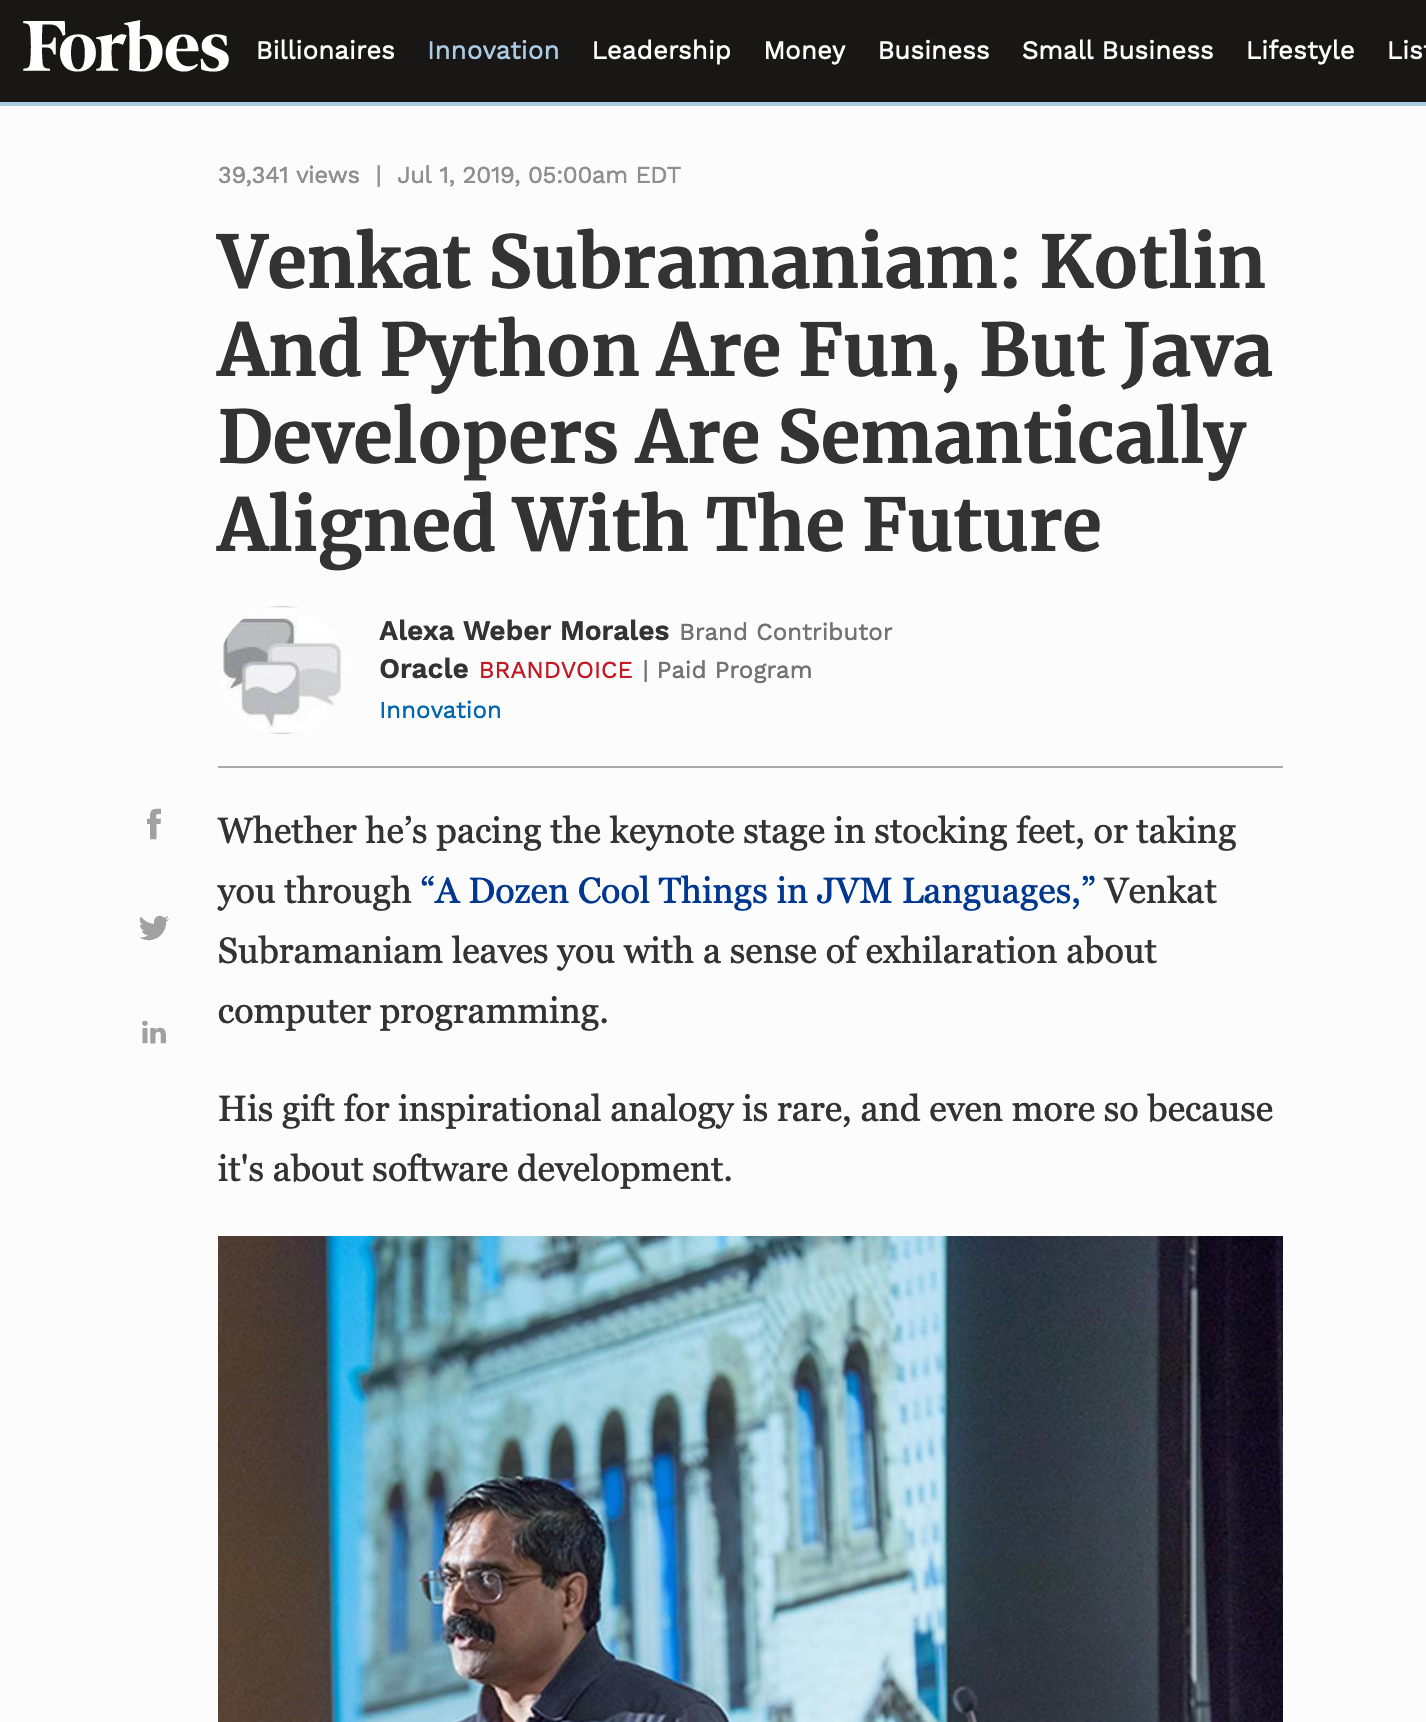
\includegraphics[width=0.5\linewidth]{Images/venkat}
    \end{figure}
\end{frame}

\begin{frame}{Curso}
	\begin{figure}
		\centering
		
\includegraphics[width=\linewidth]{Images/curso}
	\end{figure}
\end{frame}

\begin{frame}{Horarios}
	\begin{figure}
		\centering
		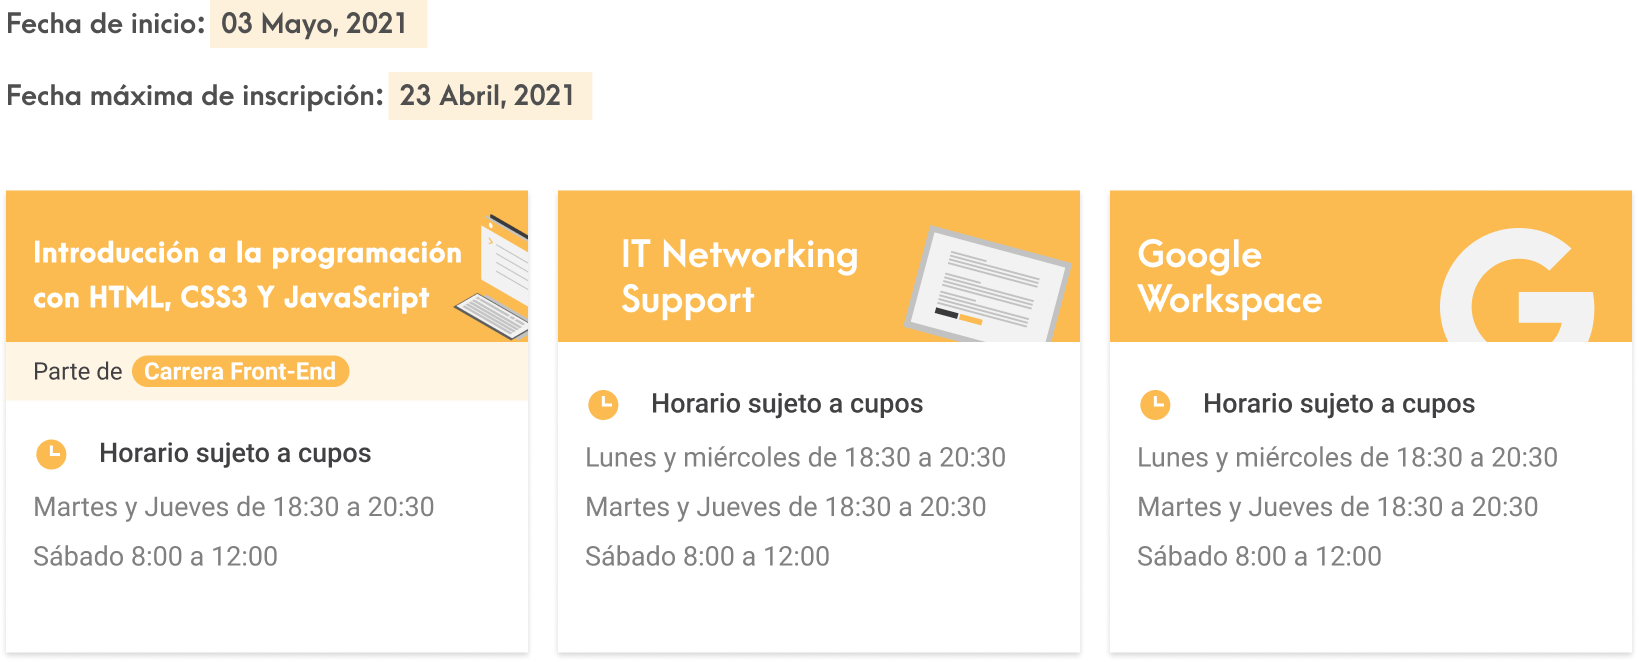
\includegraphics[width=\linewidth]{Images/horarios}
	\end{figure}
\end{frame}


{
    \usebackgroundtemplate{
\includegraphics[width=\paperwidth]{Images/final}}
    \begin{frame}
    \end{frame}
}


\end{document}

